\swjtuChapter{系统概要设计报告}

% 去掉章节前缀，使用 1 / 1.1 / 1.1.1 的编号体系
\setcounter{section}{0}
\renewcommand{\thesection}{\arabic{section}}
\renewcommand{\thesubsection}{\thesection.\arabic{subsection}}
\renewcommand{\thesubsubsection}{\thesubsection.\arabic{subsubsection}}

%%% ==================== 1 引言 ==================== %%%
\section{引言}

\subsection{编写目的}
本文档为“零售物品智能识别系统”的概要设计报告，旨在将《软件需求规格说明书》中确定的功能性与非功能性需求转化为可实施的系统体系结构、模块划分、接口契约与数据库方案。文档将作为后续详细设计、编码实现和系统测试的核心依据，确保各子系统在架构层面达成一致。

\subsection{项目背景}
本系统面向中小型零售商超场景，利用 YOLOv8 目标检测算法与计算机视觉技术，结合 Web 全栈开发能力，构建一套集“视觉导购、自助结算、智能库存管理”于一体的闭环平台。系统由四个子系统组成：Java 后端服务（retail-server）、Vue3 管理端（retail-admin-pro）、微信小程序客户端（retail-customer）以及 Python AI 服务（retail-ai），共同支撑商品管理、购物车结算、库存预警、摄像头巡检和智能搜索等核心业务。

\subsection{相关术语}
\begin{itemize}[leftmargin=2em]
  \item Spring Boot：基于 Java 的企业级应用开发框架，本系统采用 3.3 版本，运行于 Java 21 平台。
  \item MyBatis-Plus：MyBatis 的增强工具，简化数据持久层的 CRUD 操作。
  \item JWT（JSON Web Token）：一种无状态的用户鉴权令牌机制，本系统用于管理端和小程序端的登录凭证。
  \item Vue3 + Vite：前端渐进式框架与构建工具，管理端基于 TypeScript 和 Element Plus 组件库。
  \item 微信小程序：运行于微信客户端的轻应用，本系统的 C 端入口。
  \item FastAPI：Python 高性能异步 Web 框架，本系统 AI 服务的运行载体。
  \item OpenCV：开源计算机视觉库，用于摄像头采集与图像编解码。
  \item YOLOv8：新一代实时目标检测算法，用于货架商品识别。
  \item Redis：内存键值数据库，本系统用于购物车存储、Token 鉴权缓存与推荐流缓存。
  \item RESTful API：基于 HTTP 方法的资源型接口风格，系统内外部通信均采用此规范。
  \item DTO / VO：数据传输对象 / 视图对象，分别用于接收请求参数和封装响应数据。
  \item MJPEG：Motion JPEG 视频流协议，用于摄像头实时画面传输。
  \item BFF（Backend For Frontend）：为前端量身定制的后端服务层模式。
\end{itemize}

\subsection{参考文献}
\begin{enumerate}[leftmargin=2em]
  \item 《软件工程：实践者的研究方法》（第9版），Roger S. Pressman.
  \item Spring Boot 3.3 官方文档 \textnormal{https://spring.io/projects/spring-boot}
  \item Vue3 官方文档 \textnormal{https://vuejs.org/}
  \item 微信小程序开发指南 \textnormal{https://developers.weixin.qq.com/miniprogram/dev/}
  \item FastAPI 官方文档 \textnormal{https://fastapi.tiangolo.com/}
  \item YOLOv8（Ultralytics）官方文档 \textnormal{https://docs.ultralytics.com/}
  \item MyBatis-Plus 官方文档 \textnormal{https://baomidou.com/}
\end{enumerate}

%%% ==================== 2 系统体系结构设计 ==================== %%%
\section{系统体系结构设计}

\subsection{系统特点分析}
\begin{enumerate}[leftmargin=2em]
  \item \textbf{四端分离架构}：系统由 Java 后端（retail-server）、Vue3 管理前端（retail-admin-pro）、微信小程序（retail-customer）和 Python AI 服务（retail-ai）四个独立子系统组成，各自拥有独立的代码仓库、构建工具和运行环境，通过 RESTful HTTP/JSON 协议进行通信。
  \item \textbf{统一 API 网关}：retail-server 同时承担 BFF 角色，为管理端提供 \texttt{/api/*} 接口，为小程序提供 \texttt{/api/applet/*} 接口，并通过 JWT 拦截器统一鉴权。
  \item \textbf{AI 能力独立部署}：retail-ai 作为独立微服务运行在 8000 端口，仅暴露视觉识别与文本检索能力，retail-server 通过 RestTemplate 进行 HTTP 中转调用，二者可独立扩缩容。
  \item \textbf{Redis 热数据缓存}：购物车数据与推荐流等高频读写数据通过 Redis 缓存，购物车使用 Hash 结构（\texttt{cart:user:\{userId\}}）持久化，推荐流设置 TTL 自动过期，降低数据库查询压力。
  \item \textbf{定时巡检机制}：后端内置基于 ThreadPoolTaskScheduler 的摄像头定时巡检调度器，可动态调整间隔和批次大小，支持手动触发全量扫描。
\end{enumerate}

\subsection{系统体系结构设计}

\subsubsection{系统体系结构模式}
本系统整体采用\textbf{分层架构 + 微服务}的混合体系结构模式：
\begin{itemize}[leftmargin=2em]
  \item \textbf{分层架构}：retail-server 内部严格遵循 Controller → Service → Mapper 三层分层，Controller 负责请求路由与参数校验，Service 封装业务逻辑，Mapper 通过 MyBatis-Plus 完成数据持久化。
  \item \textbf{微服务拆分}：AI 视觉能力被独立为 retail-ai 微服务，与主后端通过 HTTP 协议松耦合集成，故障隔离性好。
  \item \textbf{前端 MVC/MVVM}：管理端采用 Vue3 的组合式 API + Pinia 状态管理，小程序采用微信原生框架的页面/组件模型。
  \item \textbf{BFF 模式}：retail-server 根据不同前端（管理端 / 小程序）的需求，提供差异化的接口路径和返回结构。
\end{itemize}

\subsubsection{系统体系结构设计}

\paragraph{（1）逻辑视图设计}

\begin{center}
  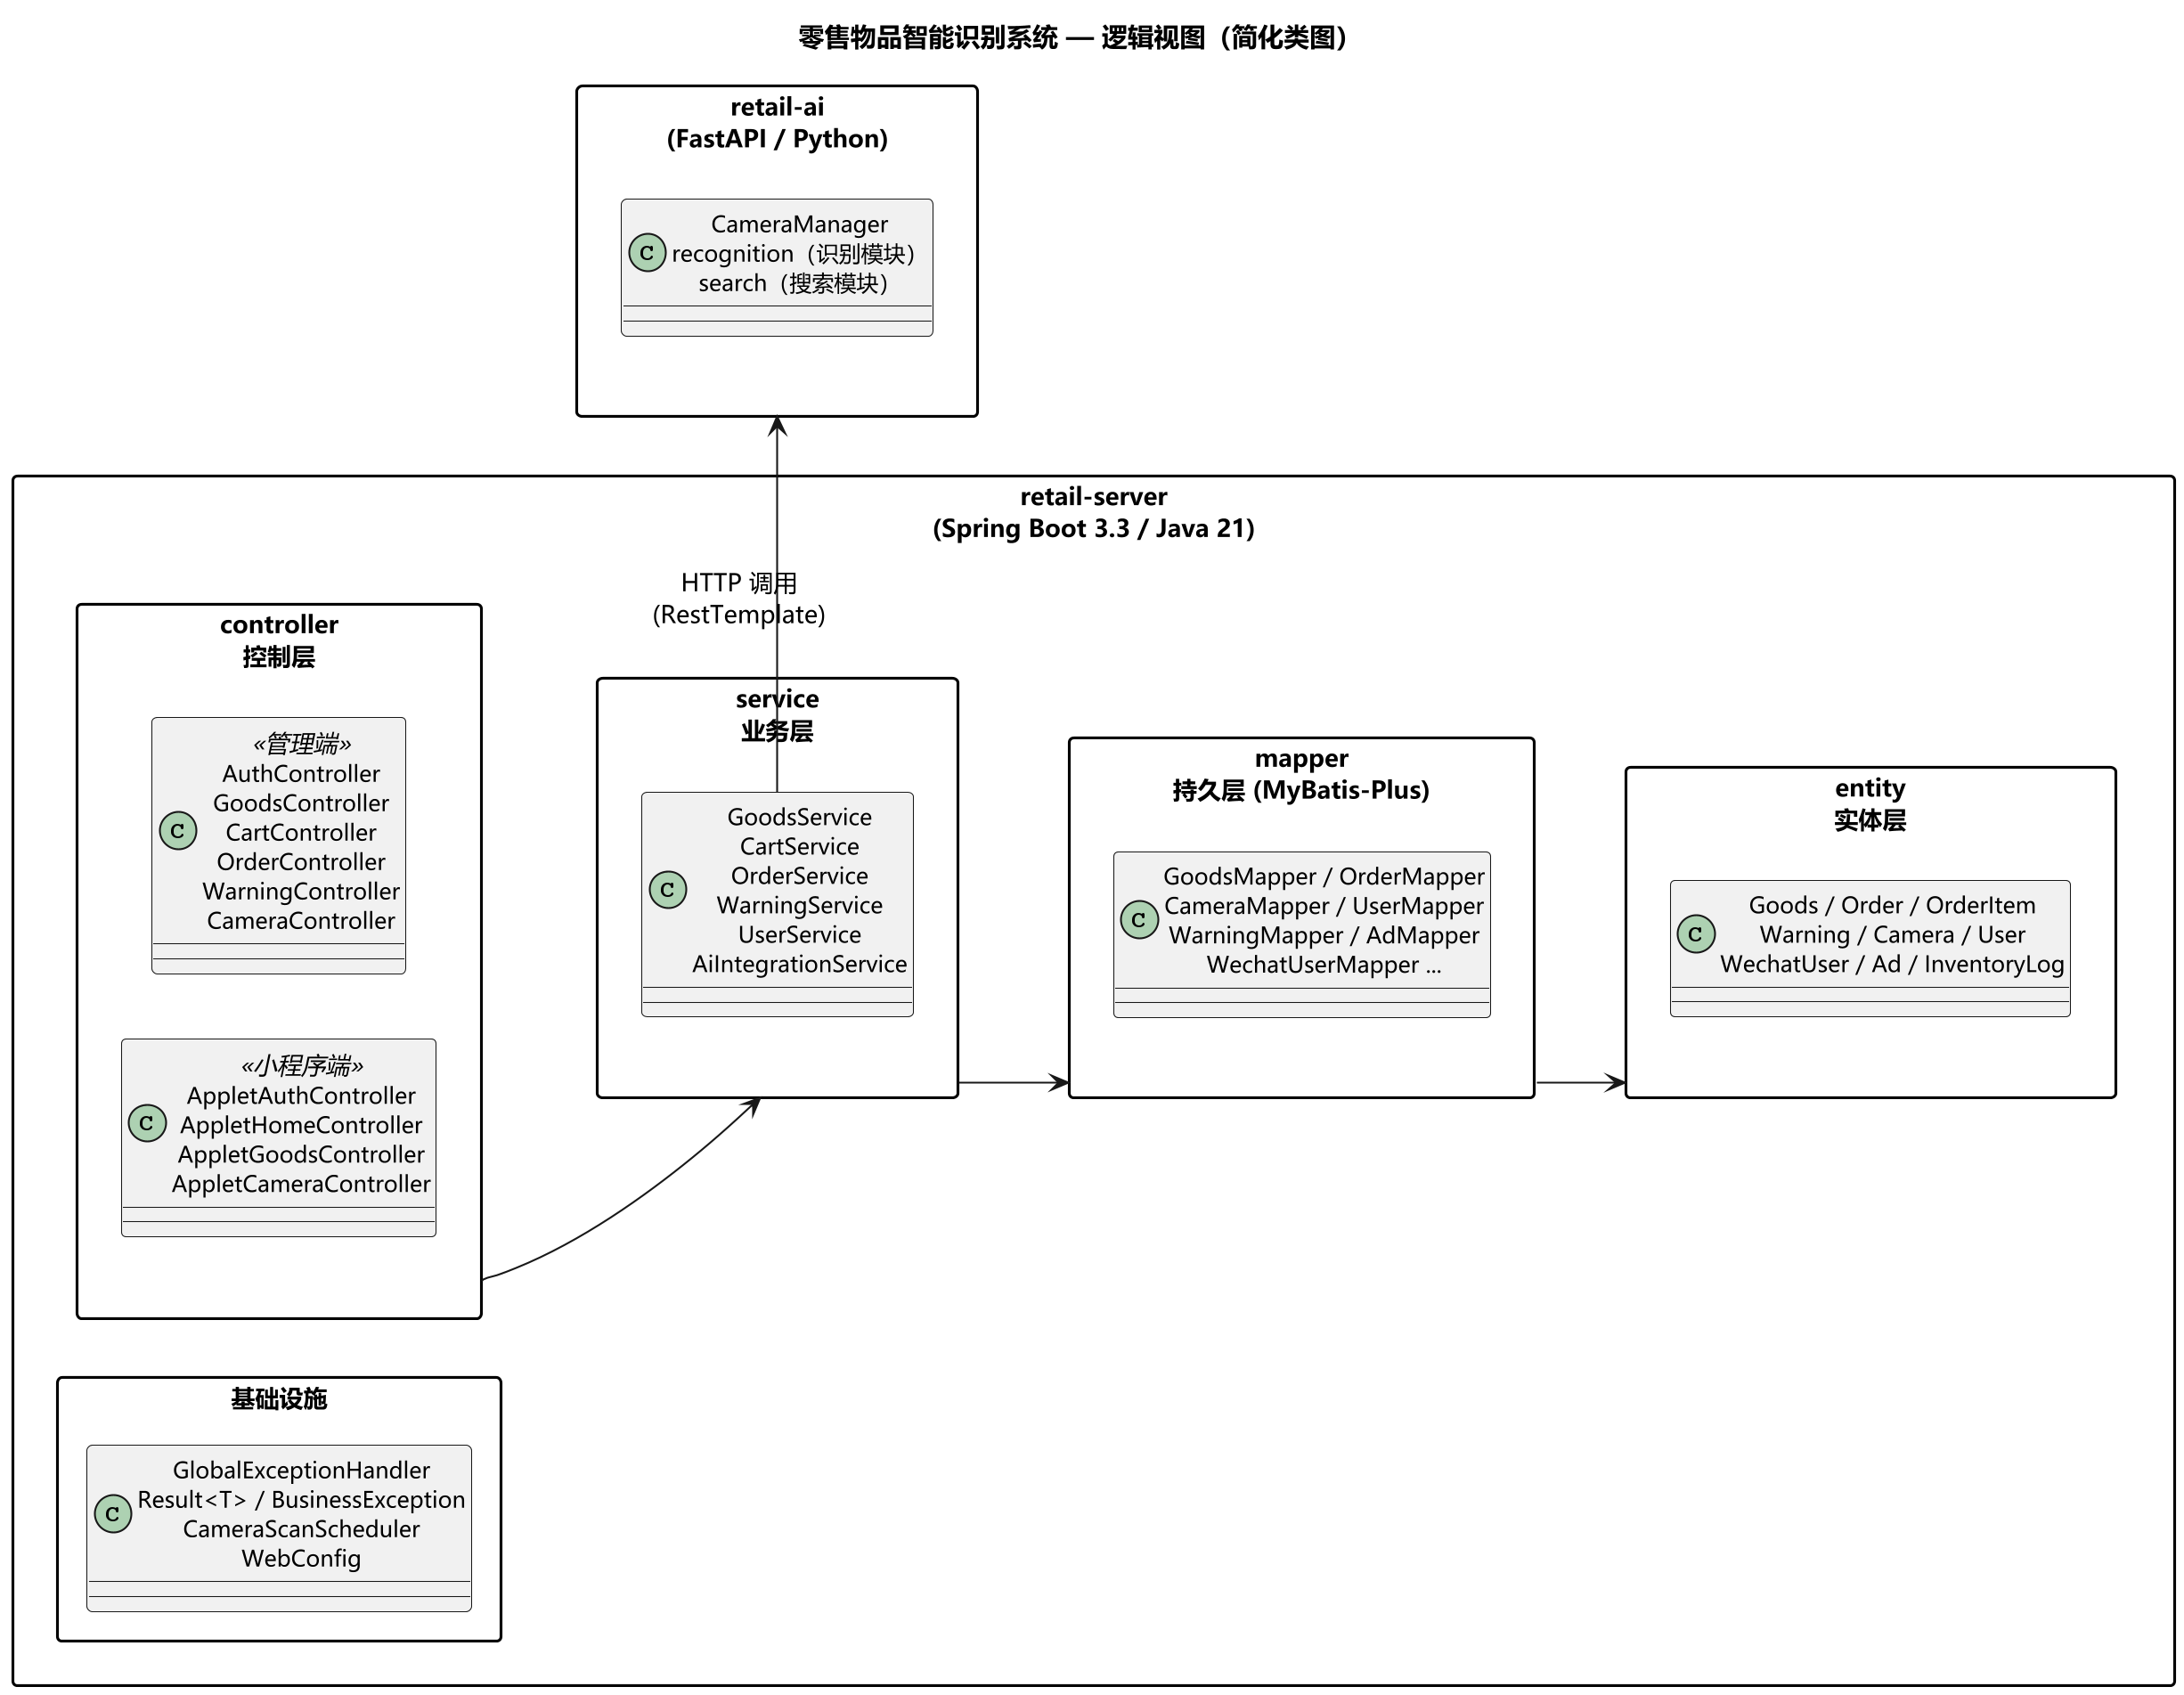
\includegraphics[width=0.95\textwidth]{images/fig-logic-view.png}\\[0.3em]
  {\zihao{-5}图2-1\quad 系统逻辑视图——简化类图}
\end{center}

retail-server 后端代码按照职责划分为以下核心包：

\begin{itemize}[leftmargin=2em]
  \item \textbf{controller 包}：面向管理端的控制器包括 AuthController（登录鉴权）、GoodsController（商品 CRUD）、CartController（购物车）、OrderController（订单结算）、WarningController（库存告警）、CameraController（摄像头管理与巡检调度）、AdminWarningController（管理端告警列表）、FileController（文件上传）；面向小程序的控制器以 \texttt{applet} 子包组织，包括 AppletAuthController、AppletHomeController、AppletGoodsController、AppletOrderController，以及 AppletCameraController（扫码识别）。
  \item \textbf{service 包}：业务逻辑层包括 GoodsService、CartService、OrderService、WarningService、UserService、OrderDetailService、AiIntegrationService（封装对 Python AI 服务的调用）及 AsyncCartService（异步购物车操作）。每个接口均有对应的 Impl 实现类。
  \item \textbf{mapper 包}：数据持久层包含 GoodsMapper、OrderMapper、OrderItemMapper、OrderDetailMapper、CameraMapper、UserMapper、WechatUserMapper、WarningMapper、InventoryLogMapper、AdMapper、GoodsCategoryMapper 共 11 个 MyBatis-Plus Mapper 接口，均继承 BaseMapper 泛型类。
  \item \textbf{entity 包}：数据实体类与数据库表一一映射，包括 Goods、Order、OrderItem、Warning、Camera、User、WechatUser、Ad、GoodsCategory、InventoryLog 等。
  \item \textbf{dto / vo 包}：DTO 用于接收前端请求（LoginRequest、CartDTO、AppletScanRequest、CameraBindRequest 等），VO 用于封装响应数据（AppletGoodsVO、CartVO、OrderVO、AppletAdVO 等）。
  \item \textbf{config 包}：全局配置类包括 WebConfig（JWT 拦截器注册与静态资源映射）、MybatisPlusConfig（分页插件）、RestTemplateConfig（HTTP 客户端）、TaskSchedulerConfig（线程池调度器）、CorsConfig（跨域配置）。
  \item \textbf{exception 包}：统一异常处理，BusinessException 为自定义业务异常，GlobalExceptionHandler 通过 \texttt{@RestControllerAdvice} 捕获所有异常并返回统一 JSON 结构。
  \item \textbf{scheduler 包}：CameraScanScheduler 实现摄像头定时巡检，支持动态配置间隔和批次大小、手动触发、生命周期管理。
  \item \textbf{common 包}：Result 类封装统一的接口返回结构（code + message + data）。
  \item \textbf{context 包}：UserContext 基于 ThreadLocal 存储当前登录用户 ID，由 JwtAuthInterceptor 在请求进入时写入。
\end{itemize}

retail-ai 服务按功能划分为三个模块：
\begin{itemize}[leftmargin=2em]
  \item \textbf{camera 模块}：CameraManager 类实现线程安全的摄像头管理（引用计数 + 空闲超时回收），camera routes 提供探测可用摄像头、单帧获取、MJPEG 视频流、资源释放等端点。
  \item \textbf{recognition 模块}：detector 模块封装 YOLO 目标检测逻辑（演示环境为模拟检测器），recognition routes 提供中心点识别和批量货架识别两个端点。
  \item \textbf{search 模块}：search routes 提供基于 Jaccard 相似度的文本关键词检索端点。
\end{itemize}

\vspace{1em}
\paragraph{（2）开发及运行视图设计}

\begin{center}
  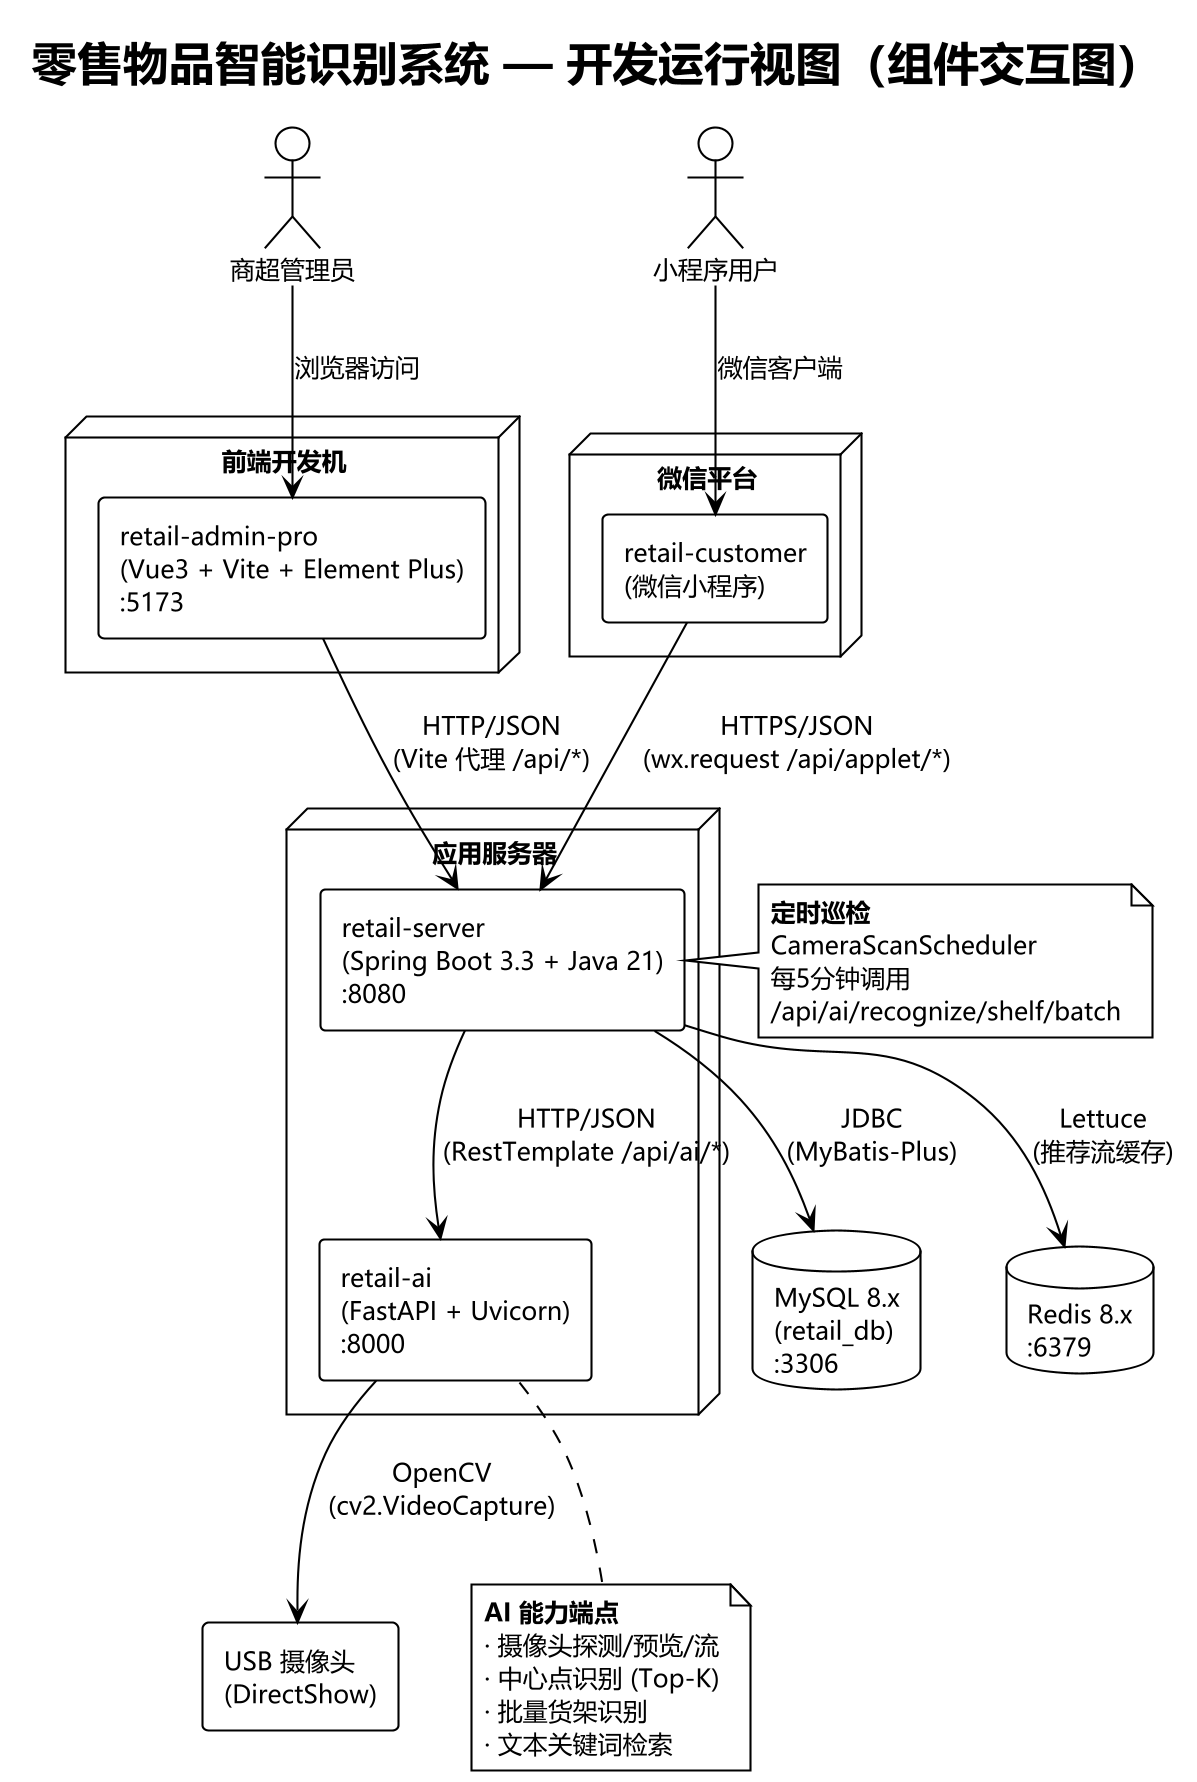
\includegraphics[width=0.95\textwidth]{images/fig-component-view.png}\\[0.3em]
  {\zihao{-5}图2-2\quad 系统开发运行视图——组件交互图}
\end{center}

系统开发与运行视图从子系统交互维度展示了四端之间的协作关系：

\begin{itemize}[leftmargin=2em]
  \item \textbf{retail-admin-pro}（Vue3 + Vite，开发端口 5173）：通过 Vite 反向代理将 \texttt{/api} 请求转发至 retail-server:8080。构建工具为 pnpm + Vite，使用 TypeScript 编写，集成 Element Plus 组件库、Axios HTTP 客户端、Pinia 状态管理和 Vue Router 路由。
  \item \textbf{retail-customer}（微信小程序）：运行于微信客户端，通过 \texttt{wx.request} 调用 retail-server 的 \texttt{/api/applet/*} 接口。使用微信原生框架，页面包括首页（index）、搜索（search）、购物车（cart）、扫码（scan）、用户中心（user）、订单（order）、商品详情（goods）、充值（recharge）、支付（payment）等。
  \item \textbf{retail-server}（Spring Boot 3.3 + Java 21，端口 8080）：通过 Maven 构建，依赖 spring-boot-starter-web、mybatis-plus-spring-boot3-starter、spring-boot-starter-data-redis、jjwt 等。启动后监听 8080 端口，接受管理端和小程序的 REST 请求。需要 AI 能力时，通过 RestTemplate 以同步 HTTP 调用 retail-ai。内置 CameraScanScheduler 定时（默认每 5 分钟）批量调用 retail-ai 的货架识别端点进行巡检。
  \item \textbf{retail-ai}（FastAPI + Uvicorn，端口 8000）：通过 pip 安装依赖（fastapi、uvicorn、opencv-python、numpy、pydantic），启动后监听 8000 端口，仅接受来自 retail-server 的内部调用。使用 OpenCV 进行摄像头操作，通过线程安全的 CameraManager 管理摄像头生命周期。
\end{itemize}

运行时数据流如下：
\begin{enumerate}[leftmargin=2em]
  \item 用户在管理端或小程序发起请求 → 到达 retail-server 的 Controller 层。
  \item Controller 调用 Service 层执行业务逻辑，Service 层通过 Mapper 层访问 MySQL 数据库。
  \item 若业务涉及 AI 能力（文本搜索、图像识别、摄像头预览），Service 或 Controller 通过 RestTemplate 向 retail-ai 发起 HTTP 请求。
  \item retail-ai 执行视觉推理或文本检索后返回 JSON 结果。
  \item retail-server 整合数据库数据与 AI 结果，封装为统一 Result 结构返回前端。
  \item 推荐流等热点数据写入 Redis 缓存，后续请求直接从缓存读取。
\end{enumerate}

\paragraph{（3）部署视图设计}

\begin{center}
  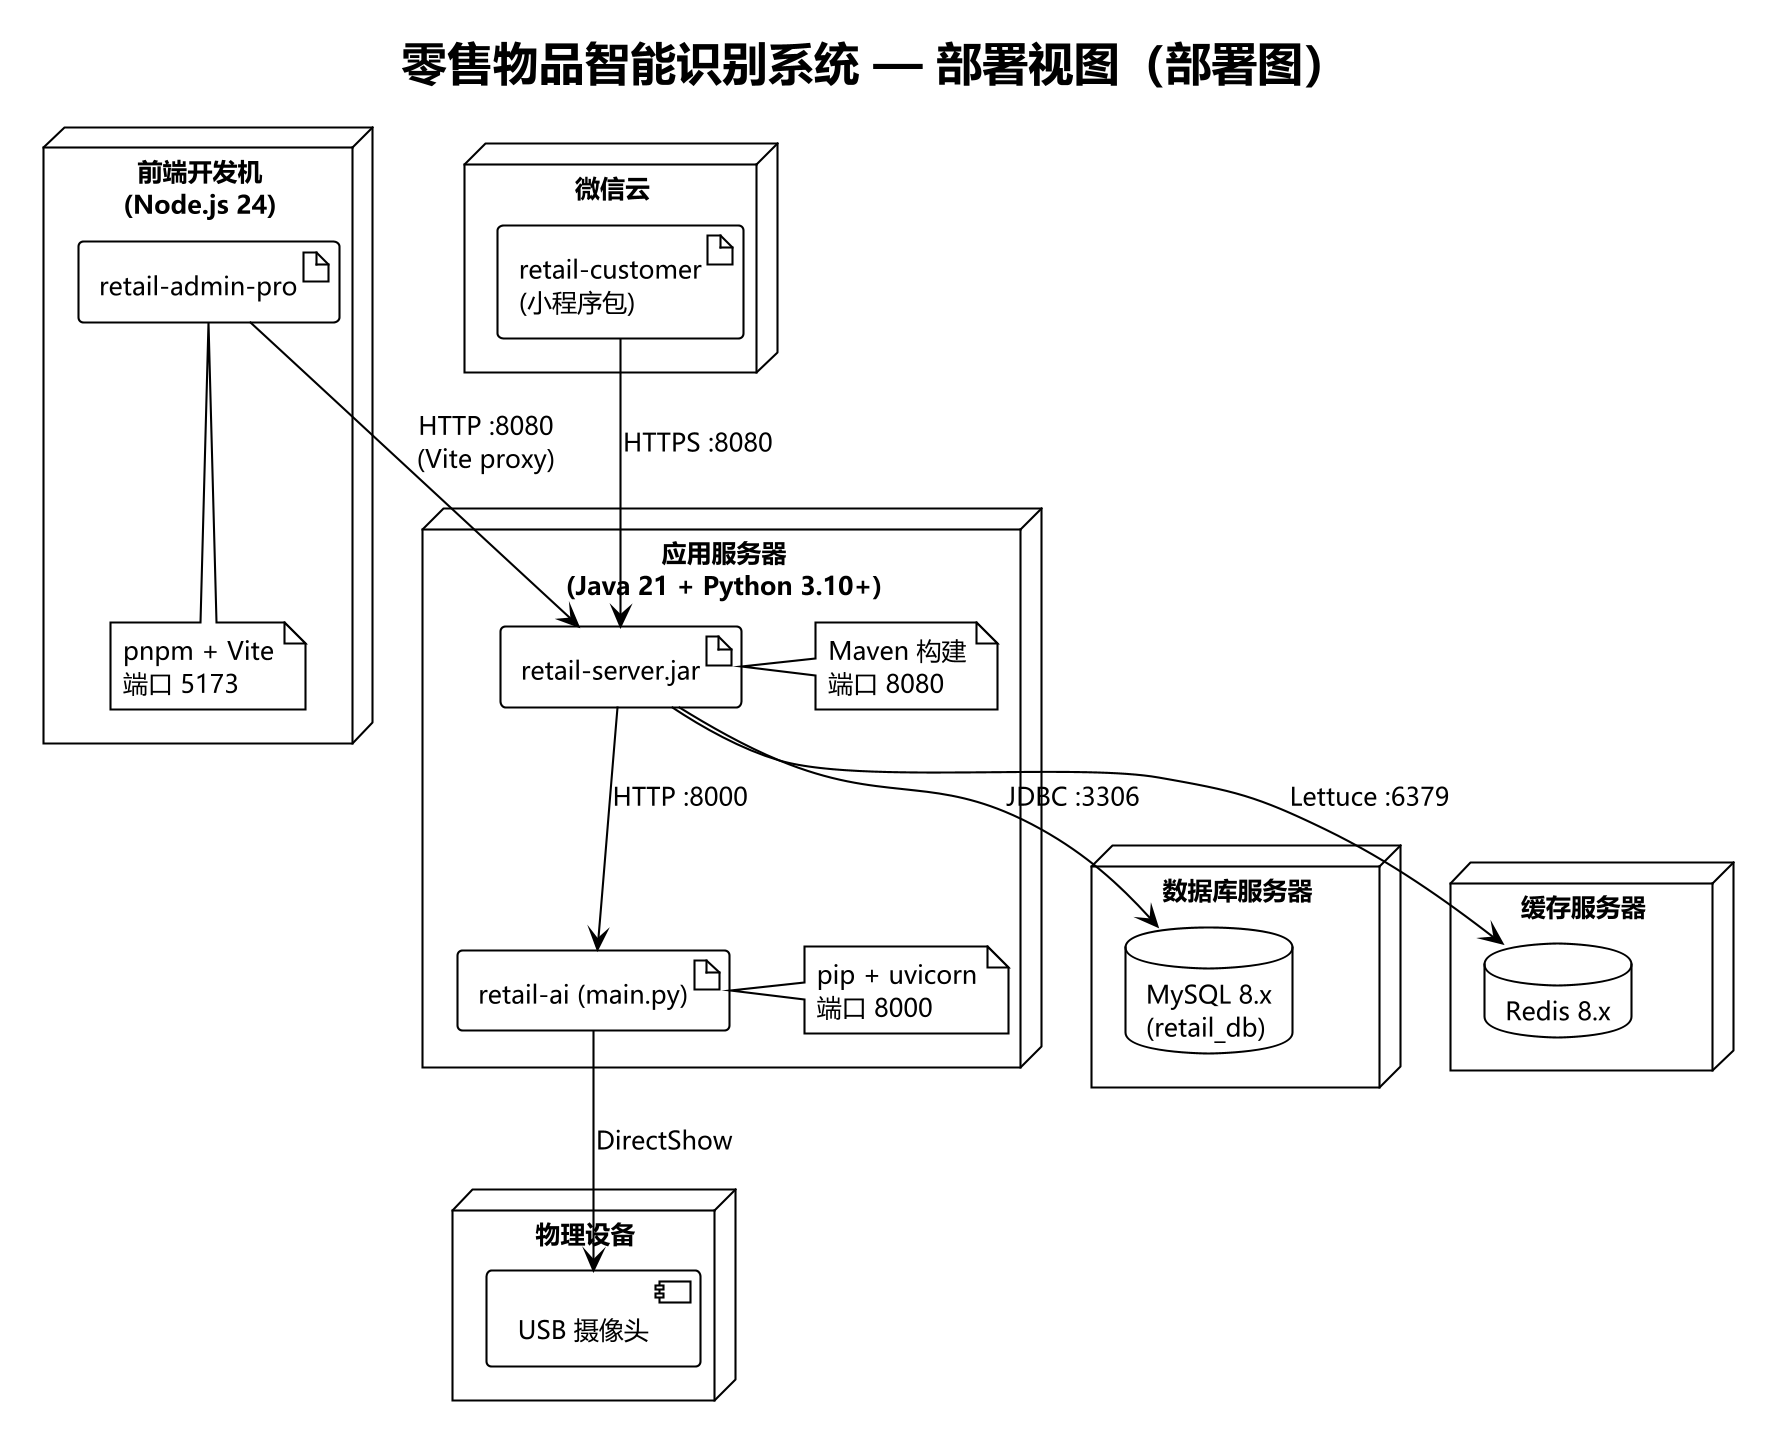
\includegraphics[width=0.88\textwidth]{images/fig-deploy-view.png}\\[0.3em]
  {\zihao{-5}图2-3\quad 系统部署视图——部署图}
\end{center}

系统各组件部署节点说明如下：

\begin{center}
  \renewcommand{\arraystretch}{1.4}
  \zihao{5}
  \begin{tabular}{|>{\centering\arraybackslash}m{2.5cm}|>{\centering\arraybackslash}m{6cm}|>{\centering\arraybackslash}m{1.5cm}|>{\centering\arraybackslash}m{2.8cm}|}
    \hline
    \textbf{部署节点} & \textbf{运行内容}                     & \textbf{端口} & \textbf{运行环境}   \\ \hline
    应用服务器         & retail-server（Spring Boot）        & 8080        & Java 21 + Maven \\ \hline
    应用服务器         & retail-ai（FastAPI + Uvicorn）      & 8000        & Python 3.10+    \\ \hline
    前端开发机         & retail-admin-pro（Vite Dev Server） & 5173        & Node.js 24      \\ \hline
    微信平台          & retail-customer（小程序包）             & —           & 微信客户端           \\ \hline
    数据库服务器        & MySQL 8.x（retail\_db 数据库）         & 3306        & —               \\ \hline
    缓存服务器         & Redis 8.x                         & 6379        & —               \\ \hline
    物理设备          & USB 摄像头                           & —           & DirectShow      \\ \hline
  \end{tabular}
  \\[0.3em]
  {\zihao{-5}表2-1\quad 系统部署节点说明}
\end{center}

部署拓扑说明：
\begin{itemize}[leftmargin=2em]
  \item 开发阶段 retail-server、retail-ai、MySQL、Redis 均可部署在同一台开发机上，管理端通过 Vite 反向代理避免跨域。
  \item 生产环境中 retail-server 与 retail-ai 建议分离部署，retail-ai 部署在配备 GPU 或摄像头的专用节点。
  \item 小程序端通过公网 HTTPS 访问 retail-server（需配置域名与 SSL 证书），管理端可通过 Nginx 部署静态资源。
  \item 摄像头设备通过 USB 连接到 retail-ai 所在节点，由 OpenCV 的 DirectShow 后端驱动采集。
\end{itemize}

%%% ==================== 3 接口设计 ==================== %%%
\section{接口设计}

\subsection{外部接口}

系统对外暴露的 RESTful API 统一采用 JSON 格式，响应结构为 \texttt{\{code, message, data\}}。以下按功能模块分组列出所有外部接口。

\paragraph{认证模块}

\begin{center}
  \renewcommand{\arraystretch}{1.4}
  \zihao{5}
  \begin{tabular}{|>{\centering\arraybackslash}m{1.5cm}|>{\centering\arraybackslash}m{5.2cm}|>{\centering\arraybackslash}m{6.0cm}|}
    \hline
    \textbf{方法} & \textbf{路径}            & \textbf{说明}            \\ \hline
    POST        & /api/auth/login        & 管理员登录，返回 JWT Token     \\ \hline
    POST        & /api/applet/auth/login & 小程序登录（微信 code 换 Token） \\ \hline
  \end{tabular}
  \\[0.3em]
  {\zihao{-5}表3-1\quad 认证模块接口}
\end{center}

\paragraph{文件管理}

\begin{center}
  \renewcommand{\arraystretch}{1.4}
  \zihao{5}
  \begin{tabular}{|>{\centering\arraybackslash}m{1.5cm}|>{\centering\arraybackslash}m{5.2cm}|>{\centering\arraybackslash}m{6.0cm}|}
    \hline
    \textbf{方法} & \textbf{路径} & \textbf{说明}    \\ \hline
    POST        & /api/upload & 上传文件，返回可访问 URL \\ \hline
  \end{tabular}
  \\[0.3em]
  {\zihao{-5}表3-2\quad 文件管理接口}
\end{center}

\paragraph{商品管理（管理端）}

\begin{center}
  \renewcommand{\arraystretch}{1.4}
  \zihao{5}
  \begin{tabular}{|>{\centering\arraybackslash}m{1.5cm}|>{\centering\arraybackslash}m{5.2cm}|>{\centering\arraybackslash}m{6.0cm}|}
    \hline
    \textbf{方法} & \textbf{路径}       & \textbf{说明}     \\ \hline
    GET         & /api/goods/page   & 分页查询商品，支持名称模糊搜索 \\ \hline
    POST        & /api/goods        & 新增商品            \\ \hline
    PUT         & /api/goods        & 修改商品（含库存补货日志记录） \\ \hline
    DELETE      & /api/goods/\{id\} & 删除商品            \\ \hline
  \end{tabular}
  \\[0.3em]
  {\zihao{-5}表3-3\quad 商品管理（管理端）接口}
\end{center}

\paragraph{购物车模块}

\begin{center}
  \renewcommand{\arraystretch}{1.4}
  \zihao{5}
  \begin{tabular}{|>{\centering\arraybackslash}m{1.5cm}|>{\centering\arraybackslash}m{5.2cm}|>{\centering\arraybackslash}m{6.0cm}|}
    \hline
    \textbf{方法} & \textbf{路径}     & \textbf{说明}  \\ \hline
    POST        & /api/cart/add   & 加入或修改购物车商品数量 \\ \hline
    GET         & /api/cart/list  & 查询当前用户购物车列表  \\ \hline
    DELETE      & /api/cart/clear & 清空当前用户购物车    \\ \hline
  \end{tabular}
  \\[0.3em]
  {\zihao{-5}表3-4\quad 购物车模块接口}
\end{center}

\paragraph{订单模块}

\begin{center}
  \renewcommand{\arraystretch}{1.4}
  \zihao{5}
  \begin{tabular}{|>{\centering\arraybackslash}m{1.5cm}|>{\centering\arraybackslash}m{5.2cm}|>{\centering\arraybackslash}m{6.0cm}|}
    \hline
    \textbf{方法} & \textbf{路径}         & \textbf{说明}  \\ \hline
    POST        & /api/order/checkout & 购物车一键结算，生成订单 \\ \hline
    GET         & /api/order/list     & 查询当前用户历史订单   \\ \hline
  \end{tabular}
  \\[0.3em]
  {\zihao{-5}表3-5\quad 订单模块接口}
\end{center}

\paragraph{库存告警模块}

\begin{center}
  \renewcommand{\arraystretch}{1.4}
  \zihao{5}
  \begin{tabular}{|>{\centering\arraybackslash}m{1.5cm}|>{\centering\arraybackslash}m{5.2cm}|>{\centering\arraybackslash}m{6.0cm}|}
    \hline
    \textbf{方法} & \textbf{路径}                 & \textbf{说明}    \\ \hline
    GET         & /api/warning/page           & 分页查询告警列表，按状态筛选 \\ \hline
    PUT         & /api/warning/\{id\}/resolve & 将告警标记为已处理      \\ \hline
    GET         & /api/admin/warning/list     & 管理端未处理告警列表     \\ \hline
  \end{tabular}
  \\[0.3em]
  {\zihao{-5}表3-6\quad 库存告警模块接口}
\end{center}

\paragraph{摄像头管理模块（管理端）}

\begin{center}
  \renewcommand{\arraystretch}{1.4}
  \zihao{5}
  \begin{tabular}{|>{\centering\arraybackslash}m{1.5cm}|>{\centering\arraybackslash}m{6cm}|>{\centering\arraybackslash}m{5.2cm}|}
    \hline
    \textbf{方法} & \textbf{路径}                           & \textbf{说明}   \\ \hline
    GET         & /api/admin/camera/list                & 查询已绑定摄像头列表    \\ \hline
    GET         & /api/admin/camera/available\_hardware & 获取可用物理摄像头索引   \\ \hline
    POST        & /api/admin/camera                     & 绑定新增摄像头       \\ \hline
    PUT         & /api/admin/camera                     & 编辑摄像头货架绑定     \\ \hline
    DELETE      & /api/admin/camera/\{id\}              & 删除摄像头         \\ \hline
    GET         & /api/admin/camera/preview/\{no\}      & 预览摄像头单帧画面     \\ \hline
    GET         & /api/admin/camera/stream/\{no\}       & MJPEG 实时视频流代理 \\ \hline
    POST        & /api/admin/camera/stream/\{no\}/stop  & 释放摄像头视频流资源    \\ \hline
  \end{tabular}
  \\[0.3em]
  {\zihao{-5}表3-7\quad 摄像头管理模块（管理端）接口}
\end{center}

\paragraph{巡检调度模块（管理端）}

\begin{center}
  \renewcommand{\arraystretch}{1.4}
  \zihao{5}
  \begin{tabular}{|>{\centering\arraybackslash}m{1.5cm}|>{\centering\arraybackslash}m{6.0cm}|>{\centering\arraybackslash}m{5.2cm}|}
    \hline
    \textbf{方法} & \textbf{路径}                         & \textbf{说明} \\ \hline
    GET         & /api/admin/camera/scheduler/config  & 查询巡检调度配置    \\ \hline
    PUT         & /api/admin/camera/scheduler/config  & 更新巡检间隔与批次   \\ \hline
    POST        & /api/admin/camera/scheduler/trigger & 手动触发全量巡检    \\ \hline
  \end{tabular}
  \\[0.3em]
  {\zihao{-5}表3-8\quad 巡检调度模块（管理端）接口}
\end{center}

\paragraph{小程序首页模块}

\begin{center}
  \renewcommand{\arraystretch}{1.4}
  \zihao{5}
  \begin{tabular}{|>{\centering\arraybackslash}m{1.5cm}|>{\centering\arraybackslash}m{6.0cm}|>{\centering\arraybackslash}m{5.2cm}|}
    \hline
    \textbf{方法} & \textbf{路径}                & \textbf{说明}     \\ \hline
    GET         & /api/applet/home/ads       & 轮播广告列表（免鉴权）     \\ \hline
    GET         & /api/applet/home/recommend & 推荐流（Redis 缓存分页） \\ \hline
  \end{tabular}
  \\[0.3em]
  {\zihao{-5}表3-9\quad 小程序首页模块接口}
\end{center}

\paragraph{小程序搜索识别模块}

\begin{center}
  \renewcommand{\arraystretch}{1.4}
  \zihao{5}
  \begin{tabular}{|>{\centering\arraybackslash}m{1.5cm}|>{\centering\arraybackslash}m{6.0cm}|>{\centering\arraybackslash}m{5.2cm}|}
    \hline
    \textbf{方法} & \textbf{路径}                 & \textbf{说明}   \\ \hline
    POST        & /api/applet/scan            & 扫码识别（返回商品详情，支持云端去重与重试）  \\ \hline
    POST        & /api/applet/goods/listByIds & 按 ID 批量查询商品详情 \\ \hline
    GET         & /api/goods/page             & 商品分页查询，支持名称模糊搜索与分类筛选 \\ \hline
  \end{tabular}
  \\[0.3em]
  {\zihao{-5}表3-10\quad 小程序搜索识别模块接口}
\end{center}

所有需要鉴权的接口（除标注“免鉴权”外）需在请求头携带 \texttt{Authorization: Bearer \{token\}}，由 JwtAuthInterceptor 统一校验。统一响应结构 Result 定义为：

\begin{center}
  \renewcommand{\arraystretch}{1.4}
  \zihao{5}
  \begin{tabular}{|>{\centering\arraybackslash}m{1.3cm}|>{\centering\arraybackslash}m{1.8cm}|>{\centering\arraybackslash}m{9.6cm}|}
    \hline
    \textbf{字段} & \textbf{类型} & \textbf{说明}                       \\ \hline
    code        & Integer     & 业务状态码（200 成功，4xx 客户端错误，5xx 服务端错误） \\ \hline
    message     & String      & 操作描述信息                            \\ \hline
    data        & T（泛型）       & 实际返回数据                            \\ \hline
  \end{tabular}
  \\[0.3em]
  {\zihao{-5}表3-11\quad 统一响应结构 Result}
\end{center}

\subsection{内部接口}

retail-server 通过 RestTemplate 以同步 HTTP 调用 retail-ai 的内部
API。这些接口不直接暴露给前端，仅用于后端服务间通信。

\begin{center}
  \renewcommand{\arraystretch}{1.4}
  \zihao{5}
  \begin{tabular}{|>{\centering\arraybackslash}m{1.5cm}|>{\centering\arraybackslash}m{6.0cm}|>{\centering\arraybackslash}m{5.2cm}|}
    \hline
    \textbf{方法} & \textbf{路径}                           & \textbf{说明}       \\ \hline
    GET         & /api/ai/cameras/available             & 探测本机可用物理摄像头索引     \\ \hline
    GET         & /api/ai/cameras/frame/\{index\}       & 获取指定摄像头单帧（base64） \\ \hline
    GET         & /api/ai/cameras/stream/\{index\}      & MJPEG 实时视频流       \\ \hline
    POST        & /api/ai/cameras/stream/\{index\}/stop & 主动释放摄像头资源         \\ \hline
    POST        & /api/ai/recognize/center              & 中心点识别 Top-K（扫码用）  \\ \hline
    POST        & /api/ai/recognize/shelf/batch         & 批量货架识别（巡检用）       \\ \hline
    POST        & /api/ai/search/text                   & 文本关键词检索商品 ID      \\ \hline
  \end{tabular}
  \\[0.3em]
  {\zihao{-5}表3-12\quad 接口接口}
\end{center}

调用约定：
\begin{itemize}[leftmargin=2em]
  \item 基础地址通过 \texttt{application.yml} 中的 \texttt{ai.service-url} 配置，默认值为 \texttt{http://localhost:8000}。
  \item 请求与响应均为 JSON 格式，Python 端使用 Pydantic 模型进行参数校验。
  \item retail-server 对 RestClientException 进行统一捕获并内置最多 2 次重试（间隔递增 1s/2s），重试耗尽后转换为 502 业务异常返回前端。
  \item 连接超时 5 秒，读取超时 60 秒（在 RestTemplateConfig 中配置）。
  \item Python AI 识别端已实现按类别去重（同一商品的多次检测仅保留距画面中心最近的一条），后端也做冗余去重校验，确保返回结果无重复商品。
\end{itemize}

%%% ==================== 4 系统数据库设计 ==================== %%%
\section{系统数据库设计}

\subsection{概念数据库设计}

\begin{center}
  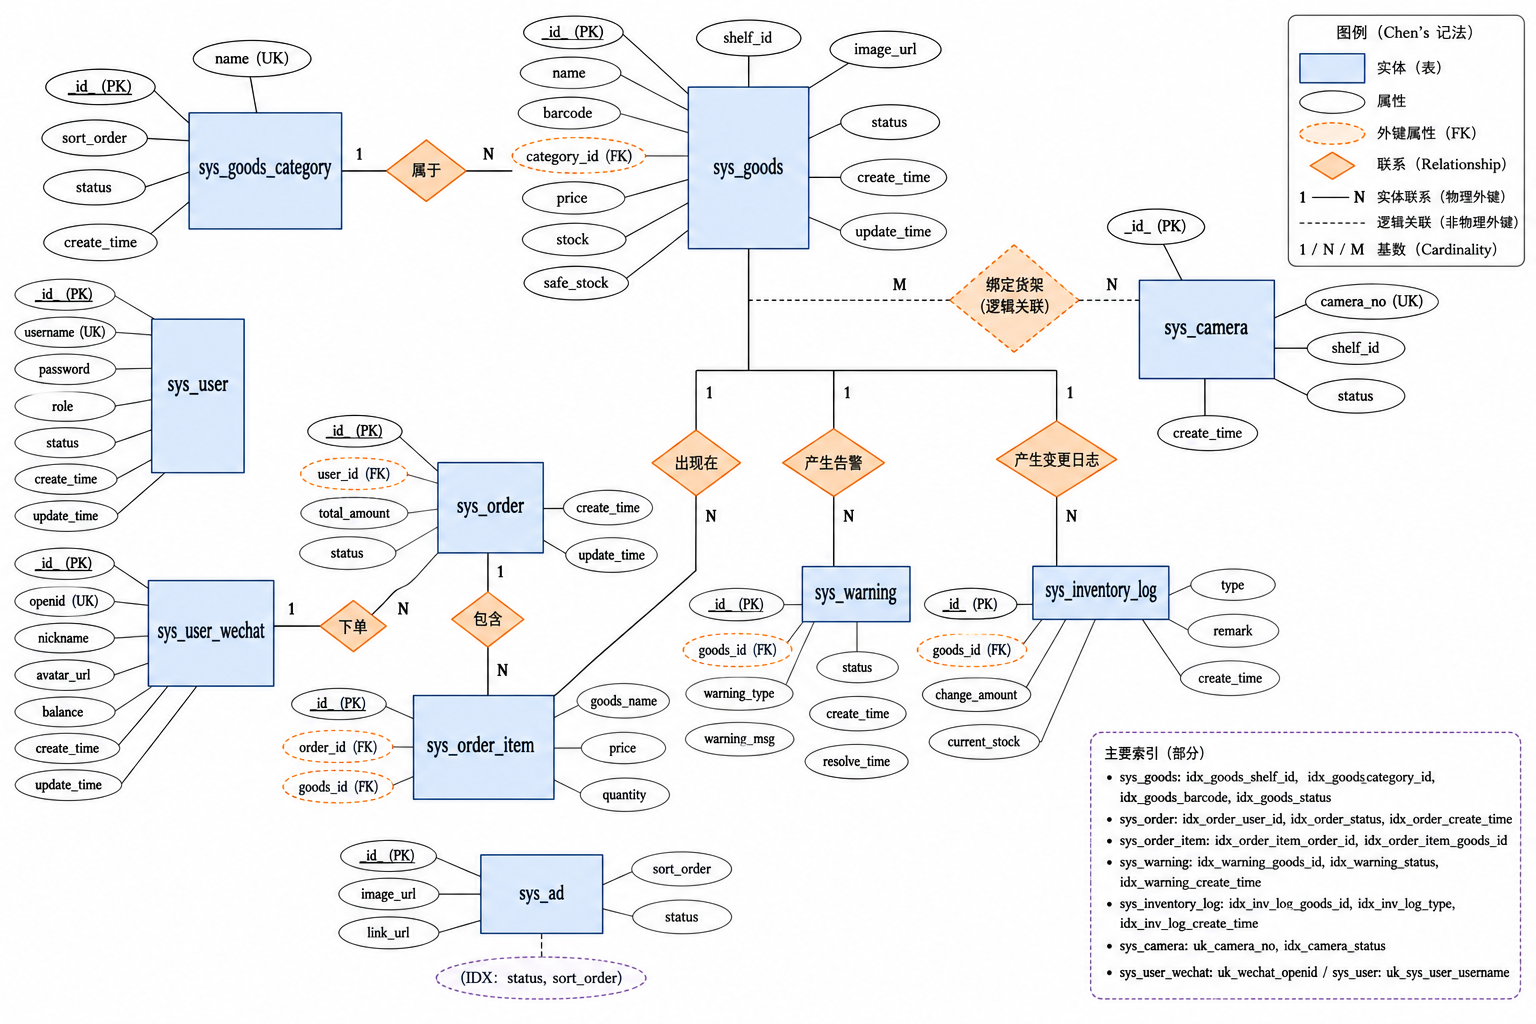
\includegraphics[width=0.95\textwidth]{images/fig-er-diagram.png}\\[0.3em]
  {\zihao{-5}图4-1\quad 系统概念数据库设计——ER 图}
\end{center}

系统数据库 \texttt{retail\_db} 共包含 10 个实体，核心实体及联系描述如下：

\begin{itemize}[leftmargin=2em]
  \item \textbf{系统用户（sys\_user）}与\textbf{订单（sys\_order）}：一对多关系，一个管理端用户可创建多个订单。
  \item \textbf{小程序用户（sys\_user\_wechat）}与\textbf{订单（sys\_order）}：一对多关系，一个小程序用户可创建多个订单。
  \item \textbf{订单（sys\_order）}与\textbf{订单明细（sys\_order\_item）}：一对多关系，一个订单包含多条明细。
  \item \textbf{商品（sys\_goods）}与\textbf{订单明细（sys\_order\_item）}：一对多关系，一个商品可出现在多条订单明细中。
  \item \textbf{商品分类（sys\_goods\_category）}与\textbf{商品（sys\_goods）}：一对多关系，一个分类下可有多个商品。
  \item \textbf{商品（sys\_goods）}与\textbf{库存告警（sys\_warning）}：一对多关系，一个商品可触发多条告警记录。
  \item \textbf{商品（sys\_goods）}与\textbf{库存变更日志（sys\_inventory\_log）}：一对多关系，一个商品有多条库存变更流水。
  \item \textbf{摄像头（sys\_camera）}与\textbf{商品（sys\_goods）}：通过 \texttt{shelf\_id} 字段逻辑关联，一个摄像头监控一个货架，一个货架上可摆放多个商品。
  \item \textbf{首页广告（sys\_ad）}：独立实体，与其他实体无外键关联。
\end{itemize}

\subsection{逻辑数据库设计}

以下按表逐一列出数据库 \texttt{retail\_db} 的全部 10 张表的逻辑结构。

\paragraph{1. 系统用户表（sys\_user）}
\begin{center}
  \renewcommand{\arraystretch}{1.4}
  \zihao{5}
  \begin{tabular}{|>{\centering\arraybackslash}m{2.5cm}|>{\centering\arraybackslash}m{3.2cm}|>{\centering\arraybackslash}m{4.4cm}|>{\centering\arraybackslash}m{3.5cm}|}
    \hline
    \textbf{字段名} & \textbf{数据类型}   & \textbf{约束}    & \textbf{说明}        \\ \hline
    id           & BIGINT UNSIGNED & PK, 自增         & 主键 ID              \\ \hline
    username     & VARCHAR(64)     & NOT NULL, UK   & 用户名                \\ \hline
    password     & VARCHAR(255)    & NOT NULL       & 密码                 \\ \hline
    role         & ENUM            & NOT NULL       & 角色（admin/customer） \\ \hline
    status       & TINYINT         & NOT NULL, 默认 1 & 状态（1 启用/0 禁用）      \\ \hline
    create\_time & DATETIME        & NOT NULL       & 创建时间               \\ \hline
    update\_time & DATETIME        & NOT NULL       & 更新时间（自动维护）         \\ \hline
  \end{tabular}
  \\[0.3em]
  {\zihao{-5}表4-1\quad sys\_user 表结构}
\end{center}

\paragraph{2. 商品分类表（sys\_goods\_category）}
\begin{center}
  \renewcommand{\arraystretch}{1.4}
  \zihao{5}
  \begin{tabular}{|>{\centering\arraybackslash}m{2.5cm}|>{\centering\arraybackslash}m{3.2cm}|>{\centering\arraybackslash}m{4.4cm}|>{\centering\arraybackslash}m{3.5cm}|}
    \hline
    \textbf{字段名} & \textbf{数据类型}   & \textbf{约束}    & \textbf{说明} \\ \hline
    id           & BIGINT UNSIGNED & PK, 自增         & 分类 ID       \\ \hline
    name         & VARCHAR(64)     & NOT NULL, UK   & 分类名称        \\ \hline
    sort\_order  & INT             & NOT NULL, 默认 0 & 排序值         \\ \hline
    status       & TINYINT         & NOT NULL, 默认 1 & 状态          \\ \hline
    create\_time & DATETIME        & NOT NULL       & 创建时间        \\ \hline
  \end{tabular}
  \\[0.3em]
  {\zihao{-5}表4-2\quad sys\_goods\_category 表结构}
\end{center}

\paragraph{3. 商品基础表（sys\_goods）}
\begin{center}
  \renewcommand{\arraystretch}{1.4}
  \zihao{5}
  \begin{tabular}{|>{\centering\arraybackslash}m{2.5cm}|>{\centering\arraybackslash}m{3.2cm}|>{\centering\arraybackslash}m{4.4cm}|>{\centering\arraybackslash}m{3.5cm}|}
    \hline
    \textbf{字段名} & \textbf{数据类型}   & \textbf{约束}     & \textbf{说明} \\ \hline
    id           & BIGINT UNSIGNED & PK, 自增          & 主键 ID       \\ \hline
    name         & VARCHAR(128)    & NOT NULL        & 商品名称        \\ \hline
    barcode      & VARCHAR(64)     & 可空, 索引          & 条形码         \\ \hline
    category\_id & BIGINT UNSIGNED & 可空, 索引          & 分类 ID       \\ \hline
    price        & DECIMAL(10,2)   & NOT NULL        & 商品价格        \\ \hline
    stock        & INT             & NOT NULL, 默认 0  & 库存数量        \\ \hline
    safe\_stock  & INT             & NOT NULL, 默认 10 & 安全库存阈值      \\ \hline
    shelf\_id    & VARCHAR(64)     & NOT NULL, 索引    & 货架编号        \\ \hline
    image\_url   & VARCHAR(255)    & 可空              & 商品图片 URL    \\ \hline
    status       & TINYINT         & NOT NULL, 默认 1  & 上/下架状态      \\ \hline
    create\_time & DATETIME        & NOT NULL        & 创建时间        \\ \hline
    update\_time & DATETIME        & NOT NULL        & 更新时间        \\ \hline
  \end{tabular}
  \\[0.3em]
  {\zihao{-5}表4-3\quad sys\_goods 表结构}
\end{center}

\paragraph{4. 订单主表（sys\_order）}
\begin{center}
  \renewcommand{\arraystretch}{1.4}
  \zihao{5}
  \begin{tabular}{|>{\centering\arraybackslash}m{2.5cm}|>{\centering\arraybackslash}m{3.2cm}|>{\centering\arraybackslash}m{4.4cm}|>{\centering\arraybackslash}m{3.5cm}|}
    \hline
    \textbf{字段名}  & \textbf{数据类型}   & \textbf{约束}  & \textbf{说明} \\ \hline
    id            & BIGINT UNSIGNED & PK, 自增       & 订单 ID       \\ \hline
    user\_id      & BIGINT UNSIGNED & NOT NULL, 索引 & 用户 ID       \\ \hline
    total\_amount & DECIMAL(10,2)   & NOT NULL     & 订单总金额       \\ \hline
    status        & VARCHAR(32)     & NOT NULL     & 订单状态        \\ \hline
    create\_time  & DATETIME        & NOT NULL, 索引 & 创建时间        \\ \hline
    update\_time  & DATETIME        & NOT NULL     & 更新时间        \\ \hline
  \end{tabular}
  \\[0.3em]
  {\zihao{-5}表4-4\quad sys\_order 表结构}
\end{center}

\paragraph{5. 订单明细表（sys\_order\_item）}
\begin{center}
  \renewcommand{\arraystretch}{1.4}
  \zihao{5}
  \begin{tabular}{|>{\centering\arraybackslash}m{2.5cm}|>{\centering\arraybackslash}m{3.2cm}|>{\centering\arraybackslash}m{4.4cm}|>{\centering\arraybackslash}m{3.5cm}|}
    \hline
    \textbf{字段名} & \textbf{数据类型}   & \textbf{约束}    & \textbf{说明} \\ \hline
    id           & BIGINT UNSIGNED & PK, 自增         & 明细 ID       \\ \hline
    order\_id    & BIGINT UNSIGNED & NOT NULL, 索引   & 订单 ID       \\ \hline
    goods\_id    & BIGINT UNSIGNED & NOT NULL, 索引   & 商品 ID       \\ \hline
    goods\_name  & VARCHAR(128)    & NOT NULL       & 商品名称快照      \\ \hline
    price        & DECIMAL(10,2)   & NOT NULL       & 商品单价快照      \\ \hline
    quantity     & INT             & NOT NULL, 默认 1 & 购买数量        \\ \hline
  \end{tabular}
  \\[0.3em]
  {\zihao{-5}表4-5\quad sys\_order\_item 表结构}
\end{center}

\paragraph{6. 库存告警表（sys\_warning）}
\begin{center}
  \renewcommand{\arraystretch}{1.4}
  \zihao{5}
  \begin{tabular}{|>{\centering\arraybackslash}m{2.5cm}|>{\centering\arraybackslash}m{3.2cm}|>{\centering\arraybackslash}m{4.4cm}|>{\centering\arraybackslash}m{3.5cm}|}
    \hline
    \textbf{字段名}  & \textbf{数据类型}   & \textbf{约束}    & \textbf{说明} \\ \hline
    id            & BIGINT UNSIGNED & PK, 自增         & 告警 ID       \\ \hline
    goods\_id     & BIGINT UNSIGNED & NOT NULL, 索引   & 商品 ID       \\ \hline
    warning\_type & VARCHAR(32)     & NOT NULL       & 告警类型        \\ \hline
    warning\_msg  & VARCHAR(255)    & NOT NULL       & 告警内容        \\ \hline
    status        & TINYINT         & NOT NULL, 默认 0 & 处理状态        \\ \hline
    create\_time  & DATETIME        & NOT NULL, 索引   & 创建时间        \\ \hline
    resolve\_time & DATETIME        & 可空             & 处理时间        \\ \hline
  \end{tabular}
  \\[0.3em]
  {\zihao{-5}表4-6\quad sys\_warning 表结构}
\end{center}

\paragraph{7. 库存变更日志表（sys\_inventory\_log）}
\begin{center}
  \renewcommand{\arraystretch}{1.4}
  \zihao{5}
  \begin{tabular}{|>{\centering\arraybackslash}m{2.5cm}|>{\centering\arraybackslash}m{3.2cm}|>{\centering\arraybackslash}m{4.4cm}|>{\centering\arraybackslash}m{3.5cm}|}
    \hline
    \textbf{字段名}   & \textbf{数据类型}   & \textbf{约束}  & \textbf{说明} \\ \hline
    id             & BIGINT UNSIGNED & PK, 自增       & 日志 ID       \\ \hline
    goods\_id      & BIGINT UNSIGNED & NOT NULL, 索引 & 商品 ID       \\ \hline
    change\_amount & INT             & NOT NULL     & 变动数量（正/负）   \\ \hline
    current\_stock & INT             & NOT NULL     & 变动后当前库存     \\ \hline
    type           & VARCHAR(32)     & NOT NULL, 索引 & 日志类型        \\ \hline
    remark         & VARCHAR(255)    & 可空           & 备注          \\ \hline
    create\_time   & DATETIME        & NOT NULL, 索引 & 创建时间        \\ \hline
  \end{tabular}
  \\[0.3em]
  {\zihao{-5}表4-7\quad sys\_inventory\_log 表结构}
\end{center}

\paragraph{8. 小程序用户表（sys\_user\_wechat）}
\begin{center}
  \renewcommand{\arraystretch}{1.4}
  \zihao{5}
  \begin{tabular}{|>{\centering\arraybackslash}m{2.5cm}|>{\centering\arraybackslash}m{3.2cm}|>{\centering\arraybackslash}m{4.4cm}|>{\centering\arraybackslash}m{3.5cm}|}
    \hline
    \textbf{字段名} & \textbf{数据类型}   & \textbf{约束}    & \textbf{说明} \\ \hline
    id           & BIGINT UNSIGNED & PK, 自增         & 主键 ID       \\ \hline
    openid       & VARCHAR(128)    & NOT NULL, UK   & 微信用户唯一标识    \\ \hline
    nickname     & VARCHAR(64)     & 可空             & 昵称          \\ \hline
    avatar\_url  & VARCHAR(255)    & 可空             & 头像 URL      \\ \hline
    balance      & DECIMAL(10,2)   & NOT NULL, 默认 0 & 钱包余额        \\ \hline
    create\_time & DATETIME        & NOT NULL       & 创建时间        \\ \hline
    update\_time & DATETIME        & NOT NULL       & 更新时间        \\ \hline
  \end{tabular}
  \\[0.3em]
  {\zihao{-5}表4-8\quad sys\_user\_wechat 表结构}
\end{center}

\paragraph{9. 首页轮播广告表（sys\_ad）}
\begin{center}
  \renewcommand{\arraystretch}{1.4}
  \zihao{5}
  \begin{tabular}{|>{\centering\arraybackslash}m{2.5cm}|>{\centering\arraybackslash}m{3.2cm}|>{\centering\arraybackslash}m{4.4cm}|>{\centering\arraybackslash}m{3.5cm}|}
    \hline
    \textbf{字段名} & \textbf{数据类型}   & \textbf{约束}    & \textbf{说明} \\ \hline
    id           & BIGINT UNSIGNED & PK, 自增         & 主键 ID       \\ \hline
    image\_url   & VARCHAR(255)    & NOT NULL       & 轮播图 URL     \\ \hline
    link\_url    & VARCHAR(255)    & 可空             & 点击跳转链接      \\ \hline
    sort\_order  & INT             & NOT NULL, 默认 0 & 排序值         \\ \hline
    status       & TINYINT         & NOT NULL, 默认 1 & 启用状态        \\ \hline
  \end{tabular}
  \\[0.3em]
  {\zihao{-5}表4-9\quad sys\_ad 表结构}
\end{center}

\paragraph{10. 摄像头管理表（sys\_camera）}
\begin{center}
  \renewcommand{\arraystretch}{1.4}
  \zihao{5}
  \begin{tabular}{|>{\centering\arraybackslash}m{2.5cm}|>{\centering\arraybackslash}m{3.2cm}|>{\centering\arraybackslash}m{4.4cm}|>{\centering\arraybackslash}m{3.5cm}|}
    \hline
    \textbf{字段名} & \textbf{数据类型}   & \textbf{约束}    & \textbf{说明}   \\ \hline
    id           & BIGINT UNSIGNED & PK, 自增         & 摄像头 ID        \\ \hline
    camera\_no   & VARCHAR(32)     & NOT NULL, UK   & 摄像头编号         \\ \hline
    shelf\_id    & VARCHAR(64)     & NOT NULL       & 绑定货架编号        \\ \hline
    status       & TINYINT         & NOT NULL, 默认 1 & 状态（1 正常/0 停用） \\ \hline
    last\_scan\_time & DATETIME    & 可空             & 最近一次巡检时间      \\ \hline
    create\_time & DATETIME        & NOT NULL       & 创建时间          \\ \hline
  \end{tabular}
  \\[0.3em]
  {\zihao{-5}表4-10\quad sys\_camera 表结构}
\end{center}

%%% ==================== 5 系统出错处理设计 ==================== %%%
\section{系统出错处理设计}

\subsection{出错信息}

系统通过 GlobalExceptionHandler（\texttt{@RestControllerAdvice}）统一拦截所有异常，将其转换为标准 Result 结构返回，避免堆栈信息直接暴露给前端。以下为系统可能出现的出错信息一览表：

\begin{center}
  \renewcommand{\arraystretch}{1.4}
  \zihao{5}
  \begin{tabular}{|>{\centering\arraybackslash}m{1.5cm}|>{\centering\arraybackslash}m{4.8cm}|>{\centering\arraybackslash}m{5.5cm}|}
    \hline
    \textbf{业务码} & \textbf{触发场景}    & \textbf{提示信息}                           \\ \hline
    400          & 请求参数缺失或非法        & “商品 ID 不能为空”“分页参数必须大于 0”等               \\ \hline
    400          & 请求体 JSON 格式错误    & “请求体 JSON 格式错误”                         \\ \hline
    400          & camera\_no 已被绑定  & “该 camera\_no 已被绑定”                     \\ \hline
    400          & 小程序登录 code 非法    & “演示环境仅支持 code=test\_code”               \\ \hline
    401          & 未登录或 Token 过期/无效 & “未登录或Token无效”                           \\ \hline
    404          & 资源不存在            & “商品不存在或修改失败”“摄像头不存在”“告警不存在”             \\ \hline
    404          & 接口路径错误           & “接口不存在，请检查请求路径”                         \\ \hline
    405          & 请求方法不匹配          & “请求方法不支持”                               \\ \hline
    415          & Content-Type 不支持 & “Content-Type 不支持，请使用 application/json” \\ \hline
    500          & 数据库操作失败          & “新增商品失败”“处理告警失败”等                       \\ \hline
    500          & 摄像头预览数据为空        & “摄像头预览数据为空”                             \\ \hline
    500          & 未知系统异常           & “服务器内部异常”                               \\ \hline
    502          & Python AI 服务调用失败 & “调用 Python XX 服务失败”                     \\ \hline
  \end{tabular}
  \\[0.3em]
  {\zihao{-5}表5-1\quad 系统出错信息一览}
\end{center}

前端出错提示设计：
\begin{itemize}[leftmargin=2em]
  \item 管理端（retail-admin-pro）：通过 Axios 拦截器统一捕获非 200 响应，调用 \texttt{checkStatus} 函数根据 HTTP 状态码映射为 Element Plus 的 ElMessage 弹窗提示；403/404/500 等页面级错误显示专用错误页面。
  \item 小程序端（retail-customer）：在 \texttt{wx.request} 的 fail 回调和 success 中判断 \texttt{res.data.code}，非 200 时通过 \texttt{wx.showToast} 显示友好错误提示。
\end{itemize}

\subsection{补救措施}

\begin{enumerate}[leftmargin=2em]
  \item \textbf{JWT 令牌过期}：前端拦截 401 响应后自动清除本地 Token 并跳转登录页面，要求用户重新认证。管理端通过 Axios 拦截器实现，小程序端在请求封装层判断后调用 \texttt{wx.redirectTo} 跳转至登录页。
  \item \textbf{AI 服务宕机}：retail-server 对所有 RestTemplate 调用进行 try-catch 包裹，捕获 RestClientException 后返回 502 错误码。AI 服务不可用不影响商品管理、购物车、订单结算等核心功能的正常运行。
  \item \textbf{数据库事务失败}：订单结算（checkout）在 Service 层使用数据库事务，库存扣减与订单写入在同一事务中执行。若任一步骤失败，事务自动回滚，保证不出现“钱已扣但库存未减”的数据不一致。
  \item \textbf{摄像头资源泄露}：retail-ai 的 CameraManager 采用引用计数机制，每次 acquire 增加计数、release 减少计数。后台 Reaper 线程每 5 秒扫描一次，对引用计数归零且空闲超过 60 秒的摄像头自动执行硬件释放。服务关闭时 \texttt{on\_shutdown} 钩子释放所有摄像头。
  \item \textbf{Redis 缓存不可用}：推荐流接口在 Redis 无数据时返回 204（无更多数据），不影响用户使用其他功能。购物车使用 Redis 存储时，异常降级为返回空列表。
  \item \textbf{并发请求冲突}：商品库存更新通过 MyBatis-Plus 的条件更新保证数据安全；摄像头管理器内部使用 \texttt{threading.Lock} 保证线程安全。
  \item \textbf{文件上传失败}：FileController 校验上传文件大小和类型，异常时返回明确错误信息，不会导致服务崩溃。
  \item \textbf{网络中断}：前端均设置请求超时（管理端 Axios 超时配置、小程序 wx.request timeout），超时后显示“网络异常”提示，用户可手动重试。
\end{enumerate}
